\section{Prüfung HS15}
\subsection{Optik}

Man hat einen Konkavspiegel und einen Planspiegel.\\
Um die Brennweite des Konkavspiegels zu bestimmen wird eine Kerze zwischen Spiegel und Wand positioniert. Abstand Spiegel zur Wand $s_1 = b = 1.8m$, Abstand Kerze zur Wand $s_2 = 1.2m$. Es erscheint ein scharfes Bild der Kerze an der Wand. Wie gross ist die Brennweite?

\begin{align*}
g&= s_1-s_2 = 1.8m-1.2m = 0.6m\\
f&=\frac{g\cdot b}{g+b} = \frac{1.6\cdot 0.6m}{1.8m+1.6m}=0.45m
\end{align*}

Wo erscheint das Bild der Nase wenn wir den Planspiegel 15cm vor die Nase halten? Um was für ein Bild handelt es sich? Können wir das Bild deutlich sehen?

\begin{itemize}
	\itemsep0em
	\item Es gilt die Gleichung: $g=-b$ Daraus folgt das sich das Bild im Abstand $2g = 0.3m$ befindet.
	\item Planspiegel erzeugen bei einer einfachen Reflexion ein virtuelles und ein einseitig umgekehrtes (seitenverkehrtes) Spiegelbild
	\item Ja können wir, da sich das Bild mehr als 25cm vom Auge entfernt befindet.
\end{itemize}

Wo erscheint das Bild wenn man den Planspiegel durch einen Konkavspiegel ersetzt?
\begin{align*}
	b &= \frac{g\cdot f}{g-f} = -0.225m\\
	\frac{B}{G} = \frac{b}{g} &\Rightarrow B = G\cdot \frac{b}{g} = G\cdot \frac{-0.225m}{0.15m} = -G\cdot 1.5
\end{align*}
Daraus folgt, dass das Bild virtuell, um Faktor 1.5 vergrössert und aufrecht ist.

\subsection{Schwingung}
Ein gefederter Sitz $m=12.5kg$ schwingt unbelastet mit einer Periode $T_1 = 0.35s$ an einer Feder hin und her. Sitzt eine Person im Sitz ist die neue Periodendauer $T_2 = 0.9s$\\
Berechnen sie die Masse $m_a$ der Person. (Ungedämpft)
\begin{align*}
	m\ddot{x} &= -c\cdot x\\
	\omega_1&= \sqrt{\frac{c}{m}}\\
	\omega_1&= \frac{2\pi}{T_1} = \frac{2\pi}{0.35s} = 17.952 s^{-1}\\
	c&= m\cdot \omega_1^2 = 12.5kg\cdot 4028.41\frac{N}{m}\\
	\omega_2 &= \frac{2\pi}{T_2} = 6.981s^{-1}\\
	m_{tot} &=\frac{c}{\omega_2^2} = \frac{4028.41 \frac{N}{m}}{(6.981)^2} = 82.651kg\\
	m_2 &= m_{tot} - m_1 = 82.651kg-12.5kg = 70.153kg
\end{align*}

Mit welcher Arbeit $W$ muss der Sitz angeregt werden um eine Amplitude von 10cm zu erreichen?
\begin{align*}
	W&=\frac{1}{2} c\cdot x^2 = \frac{1}{2} 4028.41\frac{N}{m} \cdot (0.1m)^2 = 20.142J
\end{align*}

Welche maximale Geschwindigkeit erreicht der beladene Sitz
\begin{align*}
	x(t) &= A\sin(\omega t)\\
	\dot{x}(t) &= A\cdot \omega	\cdot \underbrace{\cos(\omega\cdot t)}_{\textrm{ maximal} =1}\\
	\dot{x}_{max} &= A\cdot \omega = 0.1m \cdot 6.981s^{-1} = 0.6981\frac{m}{s}
\end{align*}

Durch die Dämpfung gehen die Auslenkungen in $N=10$ Schwingungen auf $\frac{2}{3}$ des Anfangswertes zurück. Berechnen sie den Dämpfungsgrad
\begin{align*}
	x(t) &= A\cdot e^{-\delta t} \sin(\omega \cdot t)\\
	\omega &= \sqrt{\omega_0^2 -\delta^2}\\
	e^{-\delta \cdot 10T} &= \frac{2}{3}\\
	\delta &= \frac{1}{10\cdot T} \cdot \ln(\frac{3}{2} = 0.045\frac{1}{s}
\end{align*}

\subsection{Interferenz}
Eine Seifenblase erscheint mehrfarbig obwohl die Seife farblos ist. Die Brechzahl des Seifenfilms ist $n=1.42$\\
Wie erklärt sich die Farbe Magenta\\
Durch destruktive Interferenz werden die grünen Farbanteile eliminiert. Übrig bleiben die roten und blauen Anteile welche Magenta ergeben.\\
Welche Dicke $d$ muss der Seifenfilm mindestens haben, dass für eine Wellenlänge $\lambda = 530nm$ destruktive Interferenz auftritt. Dies unter senkrechtem Lichteinfall.
\begin{align*}
k\cdot 2d -\pi &= (2m+1)\pi \quad  \textrm{ oder } n \, \Delta x = (2m+1) \frac{\lambda}{2}\\
\Rightarrow \frac{2\pi}{\lambda} \cdot 2d&=  2\pi \cdot m\\
\lambda_n &= \frac{\lambda_0}{n} = \frac{530nm}{1.42} = 373.239nm\\
d&= \frac{\lambda_n}{2}  = \frac{373.239nm}{2} = 186.62nm
\end{align*}	  	

\subsection{Dopplerradar}
Um die Geschwindigkeit eines Autos zu messen wird ein Dopplerradar verwendet. Dazu werden Wellen mit einer Frequenz $f=24 GHz$ ausgesendet. Wie schnell ist das Auto bei einer Frequenzdifferenz $\Delta f = 5kHz$
\begin{align*}
	f_e &= \sqrt{\frac{1+\left(\frac{u}{c}\right)^2}{\left(1-\frac{u}{c}\right)^2}}\cdot f_s\\	
	\Delta f &= f_e-f_s = \sqrt{\frac{1+\left(\frac{u}{c}\right)^2}{\left(1-\frac{u}{c}\right)^2}}\cdot f_s -f_s
\end{align*}
	Womit nach der Geschwindigkeit gesolvet werden kann.
	
Es gibt noch die Buebetrickliformle (linearisiert) die in diesem Fall auch zum richtigen Resultat führt.
\[
	v = \frac{|f_e - f_s|}{2\cdot f_s}\cdot c = \frac{5kHz}{24GHz}\cdot 300'000'000 m/s = 31.25m/s
\]

Wäre das Auto auch für eine Sendefrequenz $f_s = 1MHz$ messbar?\\
Da $\lambda = \frac{c}{f} = 300m$ wäre das Auto unsichtbar für die Welle.

\subsection{Koppelschwingung}
Zwei parallele Pendel sind über eine Feder aneinander gekoppelt. Die Massen der Pendel seien gleich. Die Federkonstante gegeben. Der Winkel $\alpha$ definiert die Ruhestellung.

\begin{minipage}{0.69\textwidth}
\begin{align*}
J_a\cdot \ddot{\varphi}_1 &= -m_1 g a_1(\varphi_1 +\alpha_1 + c \cdot h(l_0+(H(\varphi_2-\varphi_1)))\\
J_a\cdot \ddot{\varphi}_2 &= -m_2 g a_2(\varphi_2 +\alpha_2 - c \cdot h(l_0+(H(\varphi_2-\varphi_1)))\\[1em]
&\textrm{ In der Ruhelage gilt:}\\
-&m_1g \alpha_1 a_1+c h l_0 =0\\
&m_2g \alpha_2 a_2-c h l_0 =0\\[1em]
&\textrm{Damit vereinfachen sich die Bewegungsgleichungen zu:}\\
\ddot{\varphi}_1 &= -\frac{m_1 g a_1}{J_1} \varphi_1 + \frac{ch^2}{J_1} (\varphi_2 - \varphi_1)\\
\ddot{\varphi}_2 &= -\frac{m_2 g a_2}{J_2} \varphi_2 + \frac{ch^2}{J_2} (\varphi_2 - \varphi_1)\\[1em]
&\textrm{Ergibt für die Eigenkreisfrequenzen}\\
\omega_{10} &= \sqrt{\frac{m_1 g a_1}{J_1}}\qquad \omega_{20} = \sqrt{\frac{m_2 g a_2}{J_2}}\\[1em]
&\textrm{Addition der Gleichungen ergibt Gleichschwingung}\\
J(\ddot{\varphi}_1+\ddot{\varphi}_2) &= -mga(\varphi_1+\varphi_2)\\
\omega_s &=\sqrt{\frac{m g a}{J}}\\[1em]
&\textrm{Subtraktion der Gleichungen ergibt Gegenschwingung}\\
J(\ddot{\varphi}_1-\ddot{\varphi}_2) &= -mga(\varphi_1+\varphi_2)-2ch^2(\varphi_1-\varphi_2)\quad \textrm{mit } \Theta = \varphi_1 -\varphi_2\\
J\ddot{\Theta}_D &= -m g a \Theta_D -2c h^2 \Theta_D\\
\omega_D &= \sqrt{\frac{m g a + 2 ch^2}{J}}\\[1em]
&\textrm{Alle Schwingungen sind nun eine Summe der beiden Gleichungen}\\
\varphi_1(t) &=\frac{1}{2} \left(A_S \cdot \sin (\omega_s + \varphi_s) + A_D \cdot \sin( \omega_D + \varphi_D\right)\\
\varphi_2(t) &=\frac{1}{2} \left(A_S \cdot \sin (\omega_s + \varphi_s) - A_D \cdot \sin( \omega_D + \varphi_D\right)
\end{align*}
\end{minipage}
\begin{minipage}{0.29\textwidth}
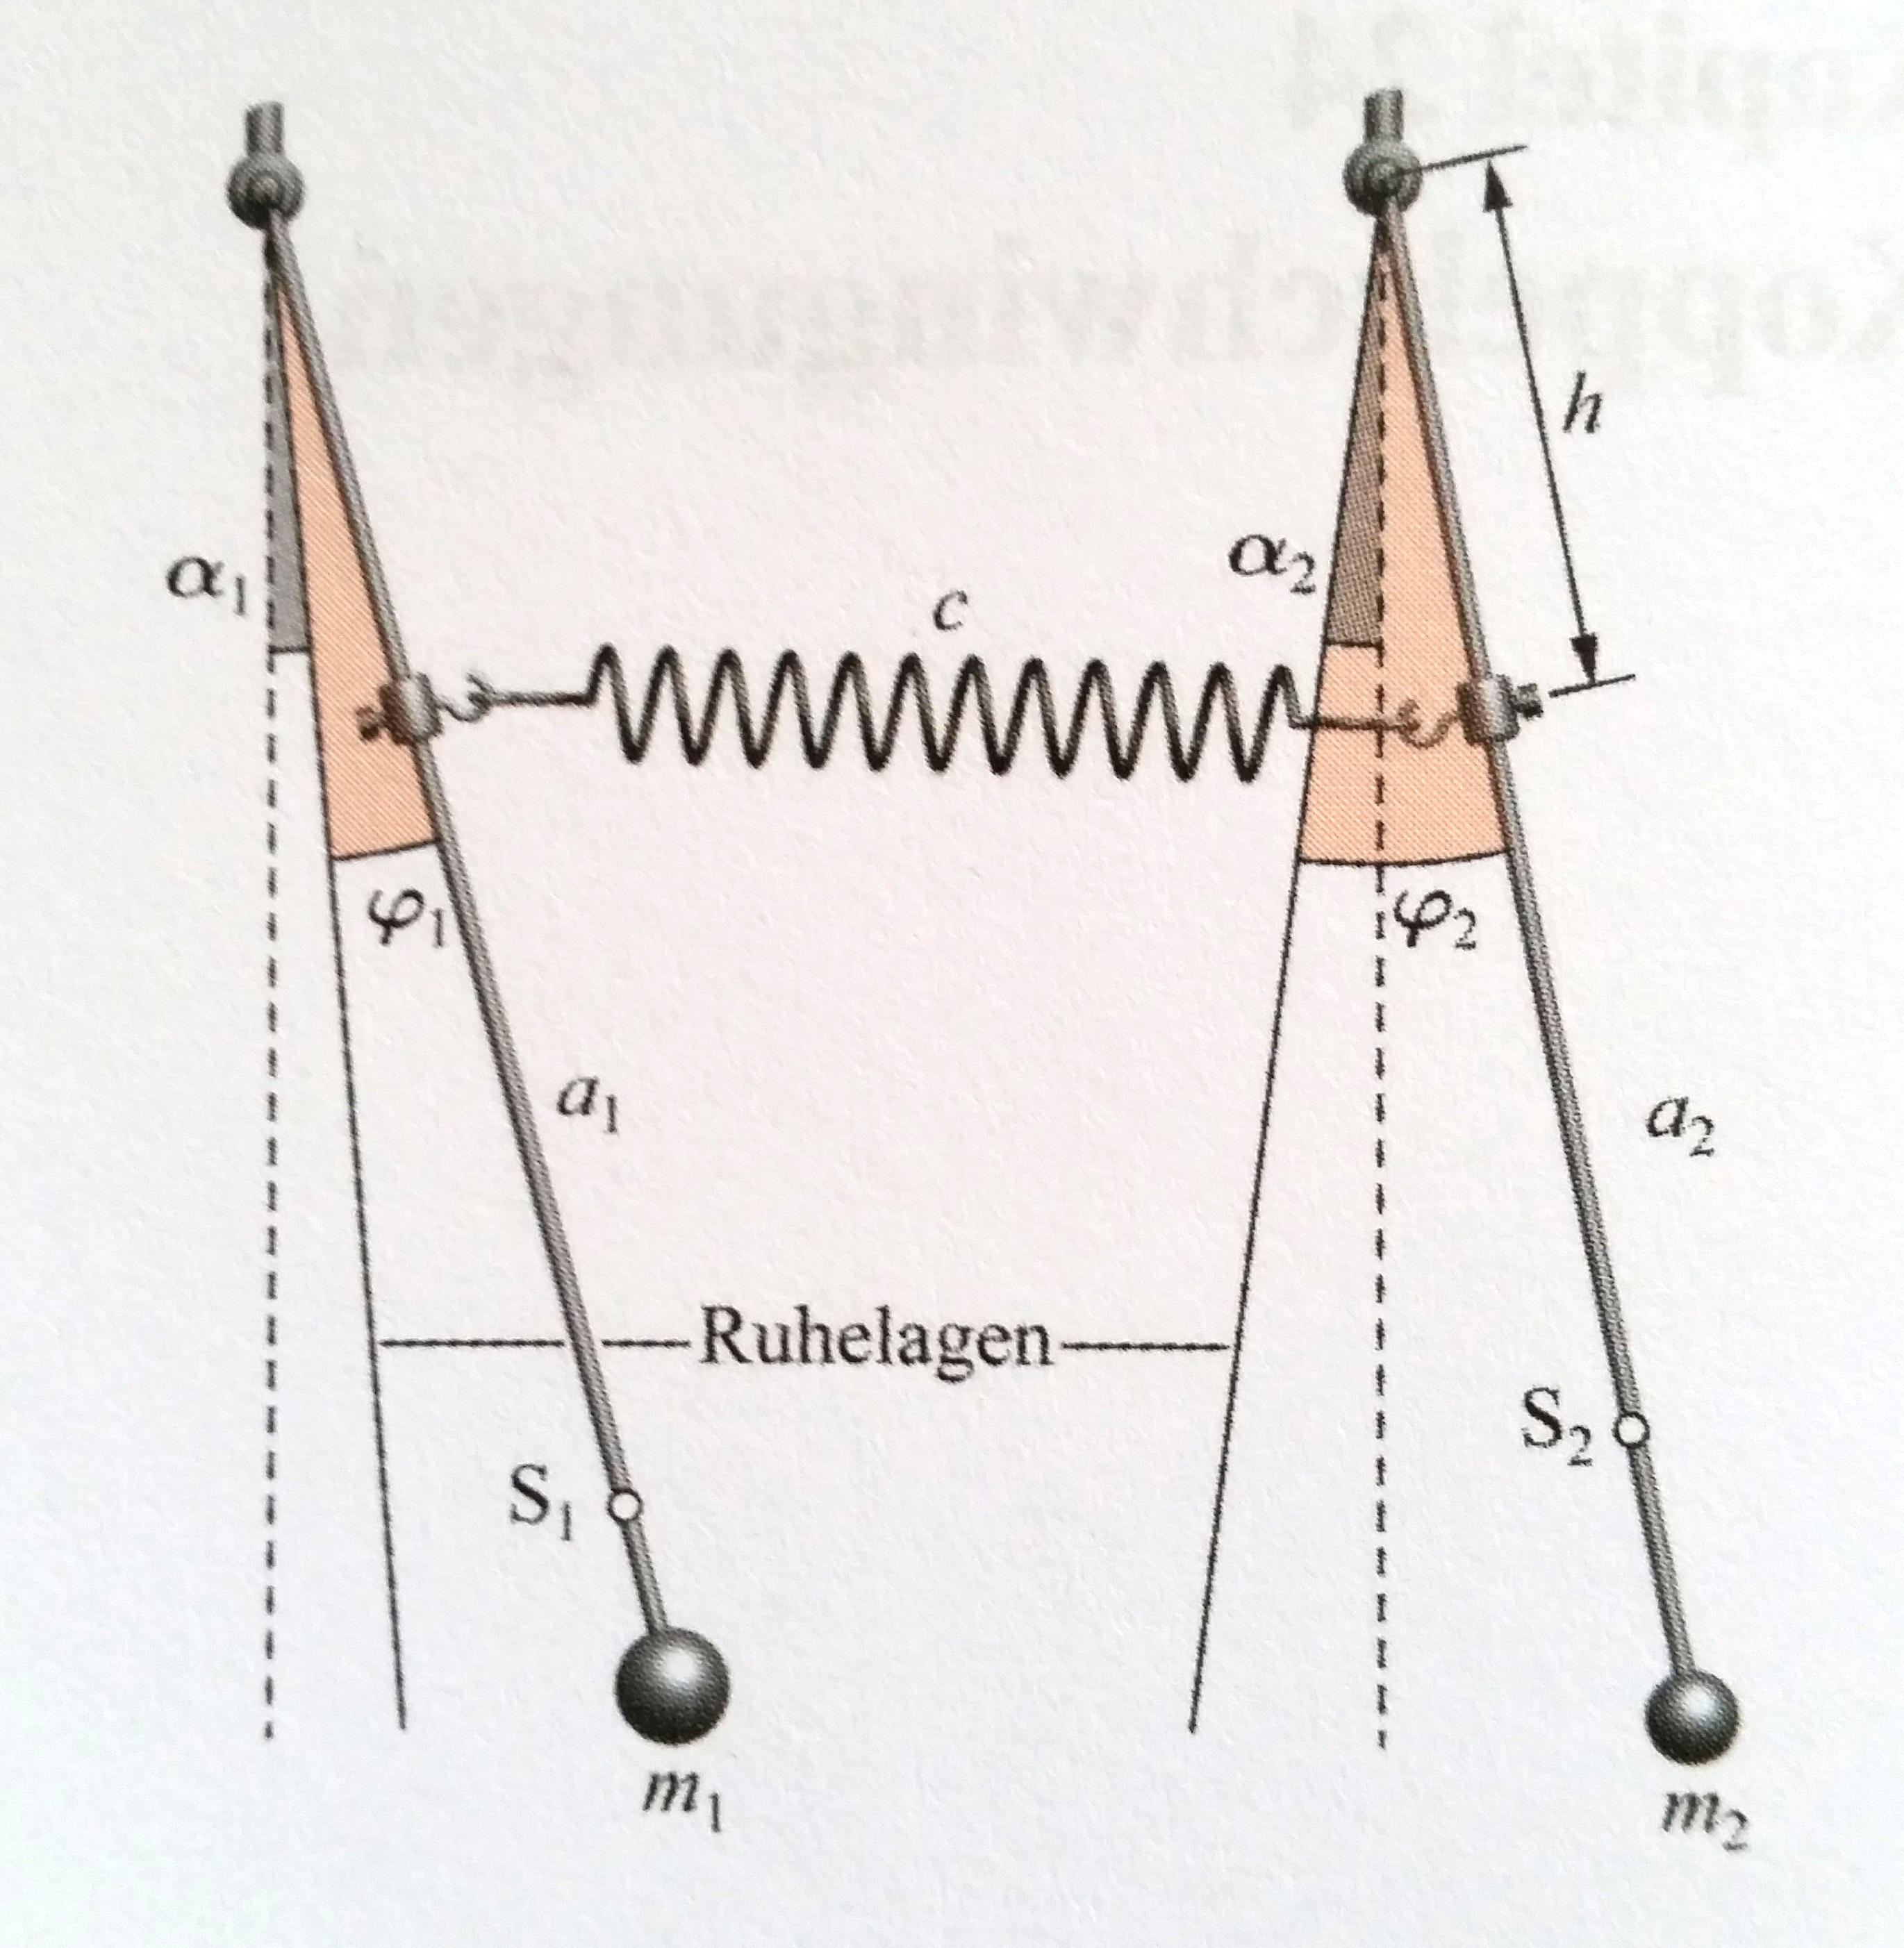
\includegraphics[width = 0.99\textwidth]{bilder/kopppendel.jpg}
\begin{itemize}
\itemsep0em
\item $J =$ Trägheitsmomente
\item $\alpha =$ Ruhelagewinkel
\item $a = $ Abstand vom Schwerpunkt zum Drehpunkt
\item $\varphi = $ Winkel gemessen ab der Ruhelage
\item $h = $ Abstand der Federbefestigung zum Drehpunkt
\item $l_0 =$ Verlängerung der Feder in Ruhelänge
\item $cl_0 = $ Vorspannung der Feder in Ruhelage
\item $A_s, A_D, \varphi_S, \varphi_D$ Aus Anfangsbedingungen
\end{itemize}
\end{minipage}